\setlength{\columnsep}{3pt}
\begin{flushleft}
	\bigskip
	You can create a private software repository that can be used everytime you want to install a package by configuring \textbf{yum server}.
	
	Below are the steps to configure a \textbf{yum server} using \textbf{FTP (file transfer protocol)}:
	
	\begin{enumerate}
		\item First attach the RHEL ISO image to the virtual machine(VM) while the machine is up and running.
		
		\begin{figure}[h!]
			\centering
			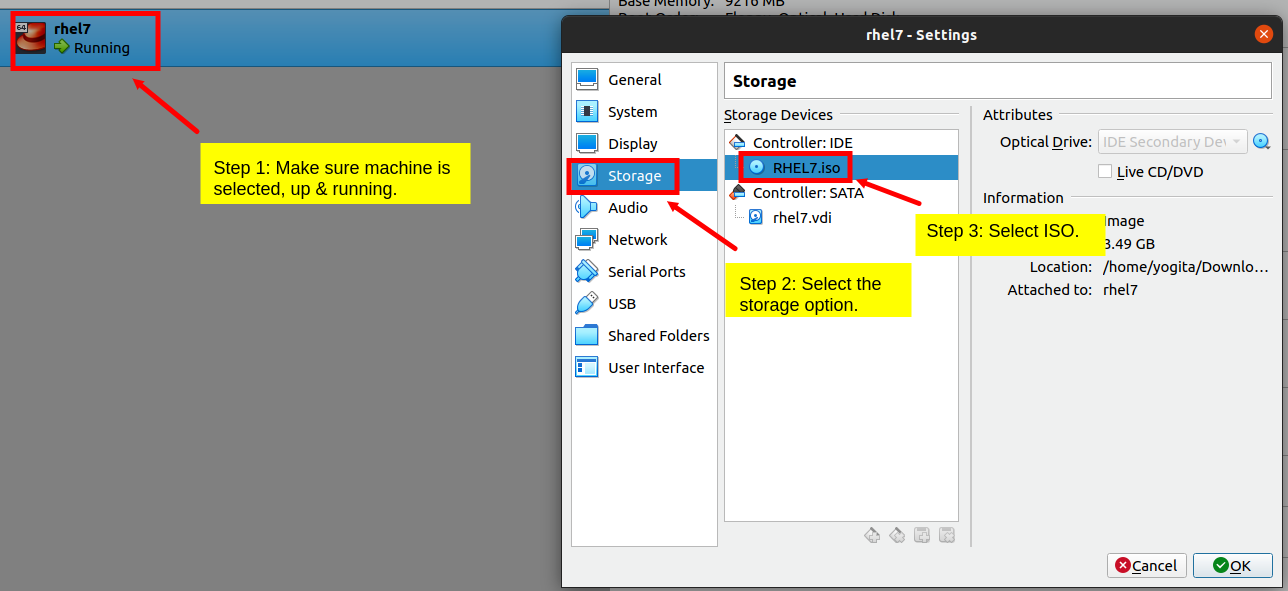
\includegraphics[scale=.3]{content/chapter11/images/ISO.png}
			\caption{Upload RHEL7 ISO}
			\label{fig:iso}
		\end{figure}	
		
		\item Unmount \textbf{/dev/sr0} \& mount the iso image attach on device \textbf{/dev/sr0} to \textbf{"/mnt"} folder.
		\begin{tcolorbox}[breakable,notitle,boxrule=-0pt,colback=black,colframe=black]
			\color{green}
			\fontdimen2\font=1em
			\# umount	/dev/sr0
			\newline
			\# mount	/dev/sr0	/mnt
			\fontdimen2\font=4pt
		\end{tcolorbox}

		\item Install following packages from attached ISO image.
		\begin{tcolorbox}[breakable,notitle,boxrule=-0pt,colback=black,colframe=black]
			\color{green}
			\fontdimen2\font=1em
			\# rpm	-ivh	/mnt/Packages/ftp-xxxx
			\newline
			\# rpm	-ivh 	/mnt/Packages/vsftpd-xxxx
			\newline
			\# rpm	-ivh	/mnt/Packages/createrepo-xxxx
			\fontdimen2\font=4pt
		\end{tcolorbox}
		
		\item Copy all packages from attached ISO image to pub directory:
		\begin{tcolorbox}[breakable,notitle,boxrule=-0pt,colback=black,colframe=black]
			\color{green}
			\fontdimen2\font=1em
			\# cp	-rv	/mnt/Packages/*	/var/ftp/pub
			\fontdimen2\font=4pt
		\end{tcolorbox}
		
		\item Create a repo in pub directory.
		\begin{tcolorbox}[breakable,notitle,boxrule=-0pt,colback=black,colframe=black]
			\color{green}
			\fontdimen2\font=1em
			\# createrepo	-v	/var/ftp/pub/
			\fontdimen2\font=4pt
		\end{tcolorbox}

		\item Start and enable the vsftpd service.
		\begin{tcolorbox}[breakable,notitle,boxrule=-0pt,colback=black,colframe=black]
			\color{green}
			\fontdimen2\font=1em
			\# systemctl   restart   vsftpd
			\newline
			\# systemctl   enable    vsftpd
			\fontdimen2\font=4pt
		\end{tcolorbox}

		\item Browse the pub directory using browser(like firefox or google chrome) with URL \textbf{ftp://(server IP address)/pub}.
		\newline
		Eg: "ftp://192.168.10.111/pub"

		\item Create a repository file named \textbf{/etc/yum.repos.d/new.repo}:
		\begin{tcolorbox}[breakable,notitle,boxrule=-0pt,colback=black,colframe=black]
			\color{white}
			\fontdimen2\font=1em
			[Title\_name] \color{yellow}  \# Add title name for this repository 
			\newline
			\color{white}
			name = Repo\_name
			\color{yellow}
  \# Add repository name
			\newline
			\color{white}
			enabled = 1
			\newline
			gpgcheck = 0
			\newline
			baseurl = ftp://(server-IP-address)/pub
			\fontdimen2\font=4pt
		\end{tcolorbox}
		\bigskip
		\begin{tcolorbox}[breakable,notitle,boxrule=-0pt,colback=yellow,colframe=yellow]
			\color{black}
			\textbf{Note:} 
			\begin{itemize}
				\item Location of repository file should be \textbf{/etc/yum.repos.d}
				\item Name of the file can be anything
				\item Extension of the file of should be \textbf{".repo"}
			\end{itemize}
		\end{tcolorbox}
		
		

		\item Clean all the cached files from any enabled repository.
		\begin{tcolorbox}[breakable,notitle,boxrule=-0pt,colback=black,colframe=black]
			\color{green}
			\fontdimen2\font=1em
			\# yum	clean	all
			\fontdimen2\font=4pt
		\end{tcolorbox}
		

		\item Refresh all the enabled repository:
		\begin{tcolorbox}[breakable,notitle,boxrule=-0pt,colback=black,colframe=black]
			\color{green}
			\fontdimen2\font=1em
			\# yum 	update 	all
			\fontdimen2\font=4pt
		\end{tcolorbox}


		\item Now you can install any packages using the YUM server.
		\newline
		Eg:
		\begin{tcolorbox}[breakable,notitle,boxrule=-0pt,colback=black,colframe=black]
			\color{green}
			\fontdimen2\font=1em
			\# yum	install	httpd -y		
			\fontdimen2\font=4pt
		\end{tcolorbox}
		

		
		
		
	\end{enumerate}

	

\end{flushleft}
\newpage



